\section{The side band ties a cut-off block}
\label{sec:sbtie}

Where a rupture splits the scene, the main band is unwrapped with a cut along the trace, and the block the cut
isolates carries an arbitrary integer. The Panama pipelines tie it with the range offsets. They read
$m = (4\pi/\lambda)\,\rho_\mathrm{off} - \phiA$, which holds the block's cycles and twice the ionosphere but no
deformation, fit a plane to $m$ 6--12\,km from the trace on each side, and compare the two planes at the trace. The
fractional parts of those ties are large: $-0.35$ (D141 on the cut of Section~\ref{sec:nisar}), $-0.13$ (D141 on the
production cut), $+0.33$ (D040), $+0.41$ (A076) and $-0.43$ (A004). This section shows that the side band ties the
block itself, and that on three of the four Panama pairs it finds those ties one cycle short. The offsets themselves
agree with it when they are read the same way. What puts the ties a cycle short is comparing two far-field planes at the
trace.

\subsection{Principle}
A block whose main-band integer is off by $\epsilon$ carries $2\pi c_0\,\epsilon = 3.21\,\epsilon$\,rad of extra raw
estimate (Table~\ref{tab:integers}): the scaled main band is taken out of the wrapped side band, so all of each wrong
cycle but $c_0$ of it wraps away. Nothing else in the raw estimate steps across the gap between two blocks. The
ionosphere is continuous across a fault zone or a strait a few kilometres wide, and the deformation is not in the
estimate. The raw estimate's step across the gap therefore measures $\epsilon$. We tile the boundary into windows of
20\,km and fit, in each,
\begin{equation}
  \hat d = P(x, y) + \delta\,\mathbf{1}_B + n, \qquad e = -\frac{\delta}{2\pi c_0},
  \label{eq:tie}
\end{equation}
over the cells of both blocks within 12\,km of the other. $P$ is a quadratic shared by both sides, so the ionosphere's
gradient and curvature are fitted across the gap rather than extrapolated from one side. The weights are each cell's
Cram\'er--Rao variance, reweighted by Tukey's biweight so that patches with local main-band cycle errors, each
3.21\,rad off, do not move the step. $e$ is the number of cycles to add to block $B$, and the tie is the median of $e$
over the windows (\texttt{split\_spectrum.\allowbreak block\_cycles}). A second estimator replaces $P$ by a Gaussian
process (Mat\'ern 3/2 plus a plane, its length and noise scales by restricted maximum likelihood in each window, the
cells as medians over $3\times3$) and checks the first.

The two ties are equally exposed to the ionosphere. A misfit of $\Delta$\,rad in the ionosphere modelled across the
gap reads as $\Delta/3.21$ cycles in the side band, and as $2\Delta/2\pi = \Delta/3.14$ cycles in $m$, which carries
the ionosphere twice and the integer at $2\pi$. They differ in everything else. The raw estimate is precise to
0.5--1\,rad per 240\,m cell and comes from the cells that make the screen. The registration offsets the pipelines tie
with are noisier, about 0.2\,m of slant range per correlation window, or 10\,rad of $m$. They are also smoothed on each
side of the trace and filled where the correlation was culled; that turns out not to matter
(Section~\ref{sec:panamaties}).

Using the bands' separation to join separately unwrapped regions is not new. \citet{libert2017split} do it at X band,
where the ionosphere is negligible, by reading each region's absolute phase from its split-band phase. At L band the
ionosphere dominates that absolute phase \citep{gomba2016toward}. What we use instead is the ionosphere's continuity
across the gap.

\subsection{Validation}
\paragraph{Synthetic ruptures.} The through-going synthetic of Section~\ref{sec:synthetic}, with the oracle main
band, so the answer is 0; three seeds, 0 and 4\,m of slip, and five variants (the default ionosphere, far-field
coherence 0.35, patchy decorrelation, travelling waves of 3\,rad at 25\,km, and a rough ionosphere of 8\,rad at 8\,km).
Putting the south block's main band one cycle off moves every one of its cells' raw estimates by exactly 3.2092\,rad,
through the whole chain, so planted ties are exact shifts: they come back to $3\times10^{-5}$ cycles.
\begin{itemize}
  \item Without local cycle errors, the polynomial reads within 0.21 of the truth (rms 0.08--0.12) in every variant but
        the rough one, and kriging within 0.11 (rms 0.03--0.06) in every one. Slip makes no difference.
  \item The rough ionosphere is where the polynomial fails. Over 20 ionospheres of each kind, with white noise in place
        of the rest of the chain, its rms is 0.09 (default), 0.11 (waves) and 0.44 (rough), where 5 of the 20 ties are
        a cycle off; kriging's is 0.02, 0.03 and 0.05, and none is off by more than 0.08.
  \item With local cycle errors in 15\% of one side's cells 2--6\,km from the gap, in 1\,km patches, the polynomial
        stays within 0.15 of the truth (0.32 in the rough ionosphere). In 35\% they bias both estimators by $+0.2$ to $+0.4$ on
        average, and a few ties come out a cycle off: the robust fit cannot reject a third of the cells that matter most.
  \item Leaving out the cells within 6\,km of the gap does not help: the extrapolation across 12\,km is worse
        (rms 0.27--0.44), with or without local errors.
\end{itemize}

\paragraph{Fake boundaries on real data.} Straight lines through one block of each of eight scenes (the four Panama
north blocks and the four Venezuela main regions), at least 15\,km from the trace, at four orientations every 12\,km,
each with the 2\,km on either side left out as a fault zone is. Nothing steps there, so every estimate should be 0.
Over 6082 windows, $|e|$ has a median of 0.035 and a 95th percentile of 0.26 (0.15 without D054), with no bias (mean
$+0.001$); 1.7\% of windows exceed 0.5. The tail has two causes, both visible in maps of the raw estimate. Most windows
that exceed 0.5 on A004, A061, A162 and D126 hold sharp-edged patches where the main band itself is off by one to
three cycles, on coastal strips, islands and a river floodplain: there the side band is right, and the fake boundary
is not a null. On D054, an evening pass, the ionosphere carries waves of 10--20\,km wavelength and several radians,
and a window whose line runs along a wave front reads up to two cycles; 4.7\% of its windows exceed 0.5. Taken as a tie is, the median over a
line's windows, no line reads a wrong integer: of 565 lines with two or more windows, the largest $|e|$ is 0.47, and
the 17.7\% of D054's lines whose windows disagree by more than 0.25, or whose median is more than 0.25 from an
integer, are flagged as ambiguous.

\paragraph{A rupture with the main band unwrapped through it.} On Venezuela's A162 and D054 the main band joins the
two sides around the rupture's west end, and the north side has data along the first 60\,km of it, so the right answer
is 0. The side band reads $+0.02$ on A162 (windows $+0.02$, $-0.04$, $+0.14$) and $-0.04$ on D054 ($+0.75$, $-0.23$,
$-0.04$), and kriging $0.00$ and $+0.03$. D054's first window sits in its ionospheric waves.

\paragraph{Two unwrappings.} D141's main band was also unwrapped without a cut, with a phase model built from the
range offsets taken out before unwrapping and put back after. That puts 92.5\% of the south block exactly two cycles
below the cut and tied unwrapping. The side band reads $+3.0$ to $+3.2$ in every window of the uncut one and $+0.6$ to
$+1.7$ in those of the tied one, whose near-fault cells carry local cycle errors the uncut one does not; their medians
differ by 1.8 (20\,km windows) to 2.1 (16\,km). Through the exact two cycles between them, the uncut unwrapping also
says the tied one needs $+1.06$.

\paragraph{Not the deformation.} Across the Panama ruptures the main band steps by $-70$ to $-208$\,rad (2--4\,km
either side) on the descending tracks and by $+125$ to $+199$\,rad on the ascending A076, while $e$ is $+1$ on all
three. A step that leaked the deformation would change sign with the look direction. The south block's offset is also
the same at every distance from the trace (Fig.~\ref{fig:tie}a), where a leak would decay with the deformation.

\subsection{The Panama ties}
\label{sec:panamaties}
Table~\ref{tab:tie} lists the south blocks of the four Panama pairs as the production screens cut them (D141, D040 and
A076 on the 20 October trace, A004 on the 13 October one). On D141, D040 and A076 the side band reads $+1.19$, $+1.28$
and $+0.93$, and kriging $+1.12$, $+1.00$ and $+0.91$. Each of the pipelines' ties is one cycle short, and the blocks'
integers are 27, 21 and $-22$. D040's polynomial median is 0.28 from an integer, because one of its three windows, at the east
end beside the trace's eastern branches, reads $+2.15$; it is flagged ambiguous, and kriging and the cells 6--12\,km from the gap
($+1.21$) agree on one cycle. A004's south block lies against the swath's near-range edge, where band A's partially
focused strip is left out, and only one window has data on both sides ($-0.30$, kriging $-0.11$): it is consistent with
the pipelines' tie but does not confirm it. On the cut of Section~\ref{sec:nisar}, D141's tie is 34, not 33.

\paragraph{The offsets agree, read the same way.} In the pipelines' geometry (a plane per side, 6--12\,km from the
trace, the two compared at it) the side band and $m$ differ by 0.6--1.5 cycles. Their combination $m + 2\hat\phi_{io}$,
which cancels both the ionosphere and the block's integer, steps by as much across the three ruptures. It looks as if
the offsets and the phase disagreed there by 7--18\,cm of range.

But read with the side band's own estimator, the same offsets agree with it (Table~\ref{tab:tie_readings}). That
estimator fits one quadratic over both blocks and a step on the south one, using cells from 2\,km of the trace. It reads
the correlator's offsets at $+0.84$, $+1.06$ and $+0.99$ cycles (the smoothed ones at $+0.84$, $+1.71$ and $+0.84$),
against the side band's $+1.19$, $+1.28$ and $+0.93$. It is the planes that differ. Each is fitted to one side alone and
extrapolated across at least 12\,km of gap. Read that way the same offsets give $+0.12$, $+0.67$ and $+0.28$ (smoothed:
$-0.08$, $+0.85$ and $+0.33$), while the side band stays at $+1.31$, $+1.44$ and $+1.00$.

A far-field plane does not carry $m$ to the trace. Within 2\,km of the trace, $m$ departs from its own far-field plane
by up to 1.0--1.5 cycles (A076, D040, A004). Used as a phase model for D141's uncut unwrapping, the offsets put the south
block two cycles from where their planes put it.

Three further checks rule out the alternatives.
\begin{itemize}
  \item \emph{The pipelines' smoothing.} The correlator's offsets before it (the ROFF lattices geocoded, with only gross
        outliers removed) match the smoothed ones to 0.3\,cm in the median (robust sd 9\,cm). They also read the same:
        $+0.84$, $+1.06$ and $+0.99$ from 2\,km.
  \item \emph{The cells.} On D141's per-pixel cells (Section~\ref{sec:pixel}), with the south block at 34, the side band
        reads $+0.37$ ($+0.11$ from 6\,km). On the cells as summed it reads $+0.19$ ($+0.10$). A bias of the summed
        cells would read $-1$.
  \item \emph{A third, independent set of offsets.} The GUNWs' own pixel offsets cannot be one here: they are not
        measurements. Their run configurations switch on ISCE3's polynomial rubbersheet, which fits one quadratic per
        frame to a $200\times200$ grid of the dense offsets, for the along-track and the slant-range offsets each, and
        resamples the secondary with it. The offset layers the products carry are that quadratic; a cubic in map
        coordinates fits them to within 3\,mm rms. They hold no coseismic step, so a tie read from them is the step left
        uncancelled, and beyond 20\,km, on coherent ground, they follow only the long-wavelength part of ours (to about
        8\,cm). The Antarctic products (Section~\ref{sec:antarctica}) take ISCE3's other branch and keep the dense
        field.
\end{itemize}
The offsets remain the weaker reading. From 6\,km they give $+0.40$, $+1.00$ and $+0.64$, and their windows scatter
several times more than the side band's (D040's run from $+0.24$ to $+4.55$). They agree with the side band, but they do
not settle the tie on their own.

\paragraph{The side band is not biased by the step.} The side band steps nowhere else: not at 565 fake boundaries, nor
across the Venezuela rupture whose integer is known. Those controls are weaker than the Panama case, though: their main
band steps by at most 26\,rad 2--4\,km from the trace, against 70--208\,rad here. A bias of the side band that grows with
the step and keeps its sign for both look directions would escape them. The Antarctic pairs of
Section~\ref{sec:antarctica} supply that control, in one look direction. Across a glacier's shear margin the
non-dispersive phase steps by 74--188\,rad. There the side band and the range offsets, read the same way, tie the cut-off
component alike, window by window: 8.95 against 8.90 cycles, and 7.97 against 7.96.

A wrong tie does not reach the slip inversion through the block's level, which a per-block offset absorbs (59\,mm per
cycle after the screen). It does through the filter, which fills the excluded zone from both blocks and mixes them
(Fig.~\ref{fig:tie}d). Correcting the three ties by a cycle raises the corrected LOS (positive toward the satellite)
just north of the trace by 36--38\,mm, by 27--29\,mm at 2--3\,km and by 8--11\,mm at 6--8\,km, and lowers it just
south by 18--20\,mm, by 10--13\,mm at 2--3\,km. The production screens carry that 5--6\,cm fake step, opposite in
sign, where the inversion reads the shallow slip.

\begin{table}[t]
\centering
\caption{The cut-off blocks' ties: cycles to add to the main band of each south block, by the side band (median over
20\,km windows of the robust polynomial, and of kriging) and by $m$ read with the same estimator (cells 2--12 and
6--12\,km from the gap), beside the range-offset tie the pipelines applied (their planes; Table~\ref{tab:tie_readings}
reads the offsets three ways). A162 and D054 are controls: their main
band runs through the rupture, and the answer is 0.}
\label{tab:tie}
\setlength{\tabcolsep}{4pt}
\begin{tabular}{lrrrrrrr}
\toprule
 & \multicolumn{2}{c}{range offsets} & \multicolumn{3}{c}{side band, $e$} & \multicolumn{2}{c}{$m$, as the side band} \\
\cmidrule(lr){2-3}\cmidrule(lr){4-6}\cmidrule(lr){7-8}
pair & tie & measured & polynomial & kriging & windows & 2--12\,km & 6--12\,km \\
\midrule
D141 & 26 & 25.87 & 1.19 & 1.12 & 2 & 0.84 & 0.19 \\
D040 & 20 & 20.33 & 1.28 & 1.00 & 3 & 1.71 & 1.03 \\
A076 & -23 & -22.59 & 0.93 & 0.91 & 4 & 0.84 & 0.57 \\
A004 & -21 & -21.43 & -0.30 & -0.11 & 1 & 0.05 & -0.16 \\
D141, Section 5's cut & 33 & 32.65 & 1.32 & -- & 2 & -- & -- \\
A162 (no cut) & -- & -- & 0.02 & 0.00 & 3 & -- & -- \\
D054 (no cut) & -- & -- & -0.04 & 0.03 & 3 & -- & -- \\
\bottomrule
\end{tabular}

\end{table}

\begin{table}[t]
\centering
\caption{The Panama ties read three ways from three fields, in cycles to add to the pipelines' offset ties (26, 20 and
$-23$). The fields are the raw dispersive estimate (the side band) and $m$, from the registration offsets as the
pipelines smoothed them and from the correlator's offsets before smoothing (gross outliers removed). Each is read with
the side band's estimator using cells from 2\,km and from 6\,km of the trace, and as the pipelines read it: a plane per
side, 6--12\,km from the trace, compared at it.}
\label{tab:tie_readings}
\small
\setlength{\tabcolsep}{3.5pt}
\begin{tabular}{lrrrrrrrrr}
\toprule
 & \multicolumn{3}{c}{side band} & \multicolumn{3}{c}{offsets, smoothed} & \multicolumn{3}{c}{offsets, raw} \\
\cmidrule(lr){2-4}\cmidrule(lr){5-7}\cmidrule(lr){8-10}
pair & 2\,km & 6\,km & planes & 2\,km & 6\,km & planes & 2\,km & 6\,km & planes \\
\midrule
D141 & 1.19 & 1.05 & 1.31 & 0.84 & 0.19 & -0.08 & 0.84 & 0.40 & 0.12 \\
D040 & 1.28 & 1.21 & 1.44 & 1.71 & 1.03 & 0.85 & 1.06 & 1.00 & 0.67 \\
A076 & 0.93 & 0.95 & 1.00 & 0.84 & 0.57 & 0.33 & 0.99 & 0.64 & 0.28 \\
\bottomrule
\end{tabular}

\end{table}

\begin{figure}[t]
\centering
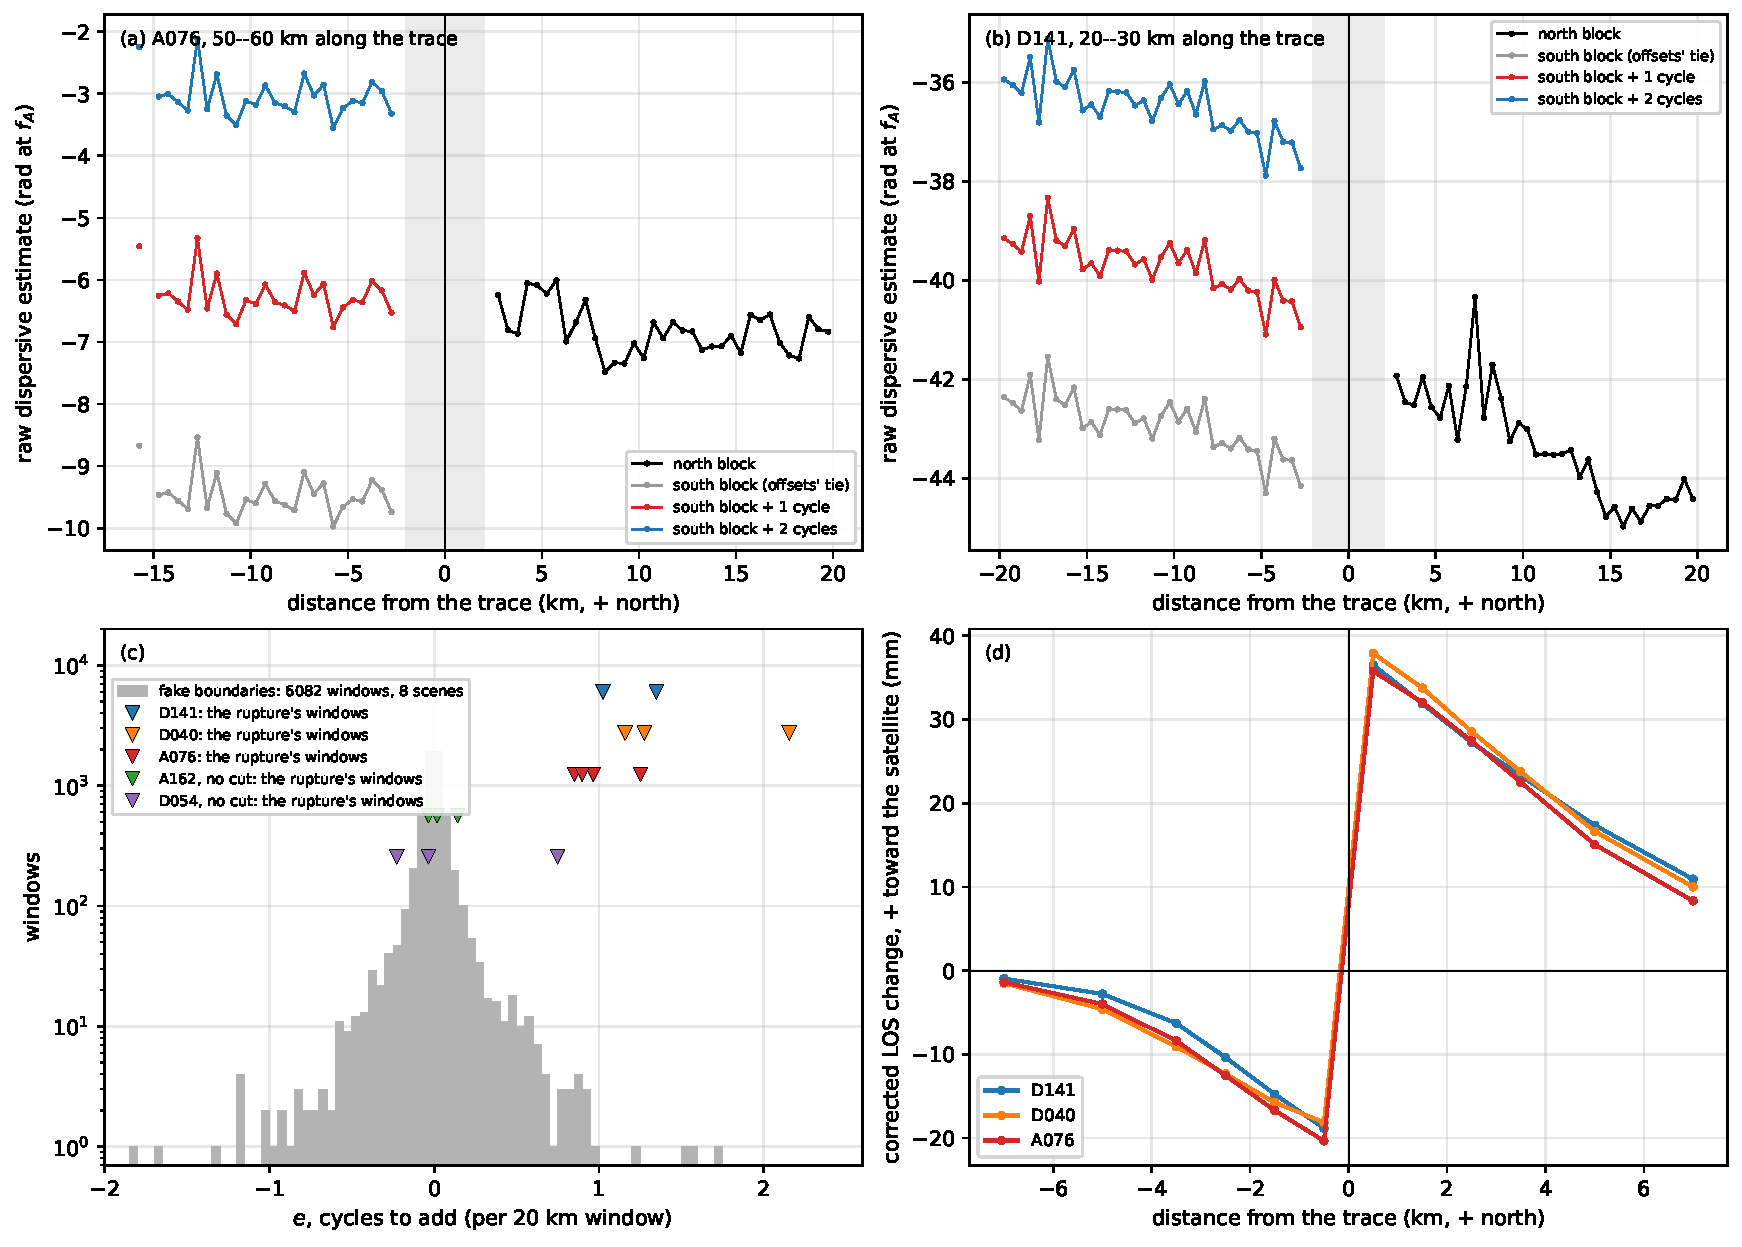
\includegraphics[width=\textwidth]{figures/fig_tie}
\caption{The side-band tie. (a, b) The raw dispersive estimate across the trace, median in 0.5\,km bins over 10\,km of
the trace, with the south block on the pipelines' offset tie and one and two cycles up. (c) $e$ on fake boundaries in eight
scenes (grey), and the windows along the real ruptures: one cycle on D141, D040 and A076, zero on the Venezuela
controls. (d) What adding one cycle to each south block does to the corrected LOS, beyond each block's constant: the
fake step the production screens carry, with the opposite sign.}
\label{fig:tie}
\end{figure}
